\mainmatter

\chapter{Fondamenti Teorici}

\section{La nascita del web}
Tim Berners-Lee, uno scienziato britannico, mentre lavorava al CERN nel 1989 sollevò un enorme problema che riguardava la condivisione di informazioni. Nonostante al CERN ci fosse una buona struttura gestionale per il raggiungimento degli obiettivi, Tim si rese conto che a causa dell'elevato turnover del personale, l'introduzione dei nuovi dipendenti richiedeva una grande quantità di tempo e molti dettagli tecnici dei progetti venivano persi o recuperati solo grazie ad un'indagine investigativa di emergenza.
Per risolvere questo problema, Tim propose nel marzo 1989 (Figura \ref{fig:proposta1989}) lo sviluppo del World Wide Web, la cui idea alla base era quella di creare un potente sistema informativo globale facile da utilizzare, unendo le tecnologie in costante evoluzione del web, con i data networks e gli hypertext.

La proposta fu definita \textit{"vaga ma eccitante"} dal suo capo, che nonostante lo scetticismo gli diede la possibilità di lavorarci nel settembre 1990.\\
Tim iniziò delineando le tre tecnologie che sono le fondamenta del web ancora oggi:
\begin{itemize}
\item HTML (HyperText Markup Language)
\item URI (Uniform Resource Identifier): un indirizzo che identifica ogni risorsa nel web, solitamente chiamato URL.
\item HTTP (HyperText Transfer Protocol): il protocollo che permette di recuperare le risorse all'interno del web.
\end{itemize}
Due mesi dopo, insieme all'ingegnere Robert Caillaiu, la proposta venne formalizzata delineando i concetti principali e i termini importanti sul Web (Figura \ref{fig:proposta1990}).
Alla fine del 1990 Tim Berners-Lee aveva realizzato il primo browser e Web server funzionanti.
La prima pagina web conteneva le informazioni del progetto WWW, con tutti i dettagli tecnici per la creazione di un web server e come collegarlo ad altri web server.
La creazione di questo progetto risolse il problema del recupero delle informazioni, garantendone un facile accesso.\cite{historyOfWeb}\cite{historyOfWeb2}

\begin{figure}
\centering
     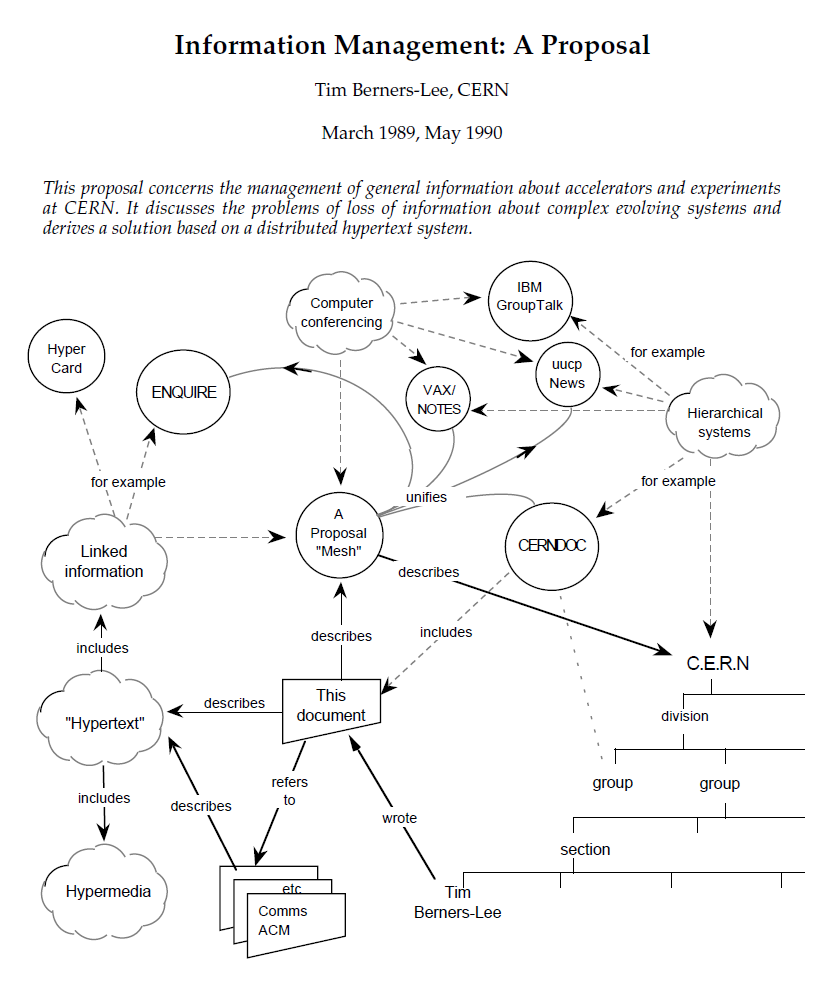
\includegraphics[width=1.0\textwidth]{images/proposta-web-1989.png}
    \caption{Prima pagina della proposta di Tim-Berners-Lee per il World Wide Web}
    \label{fig:proposta1989}
    \cite{propostaWWW1989}
    
\end{figure}

\begin{figure}
    \centering
    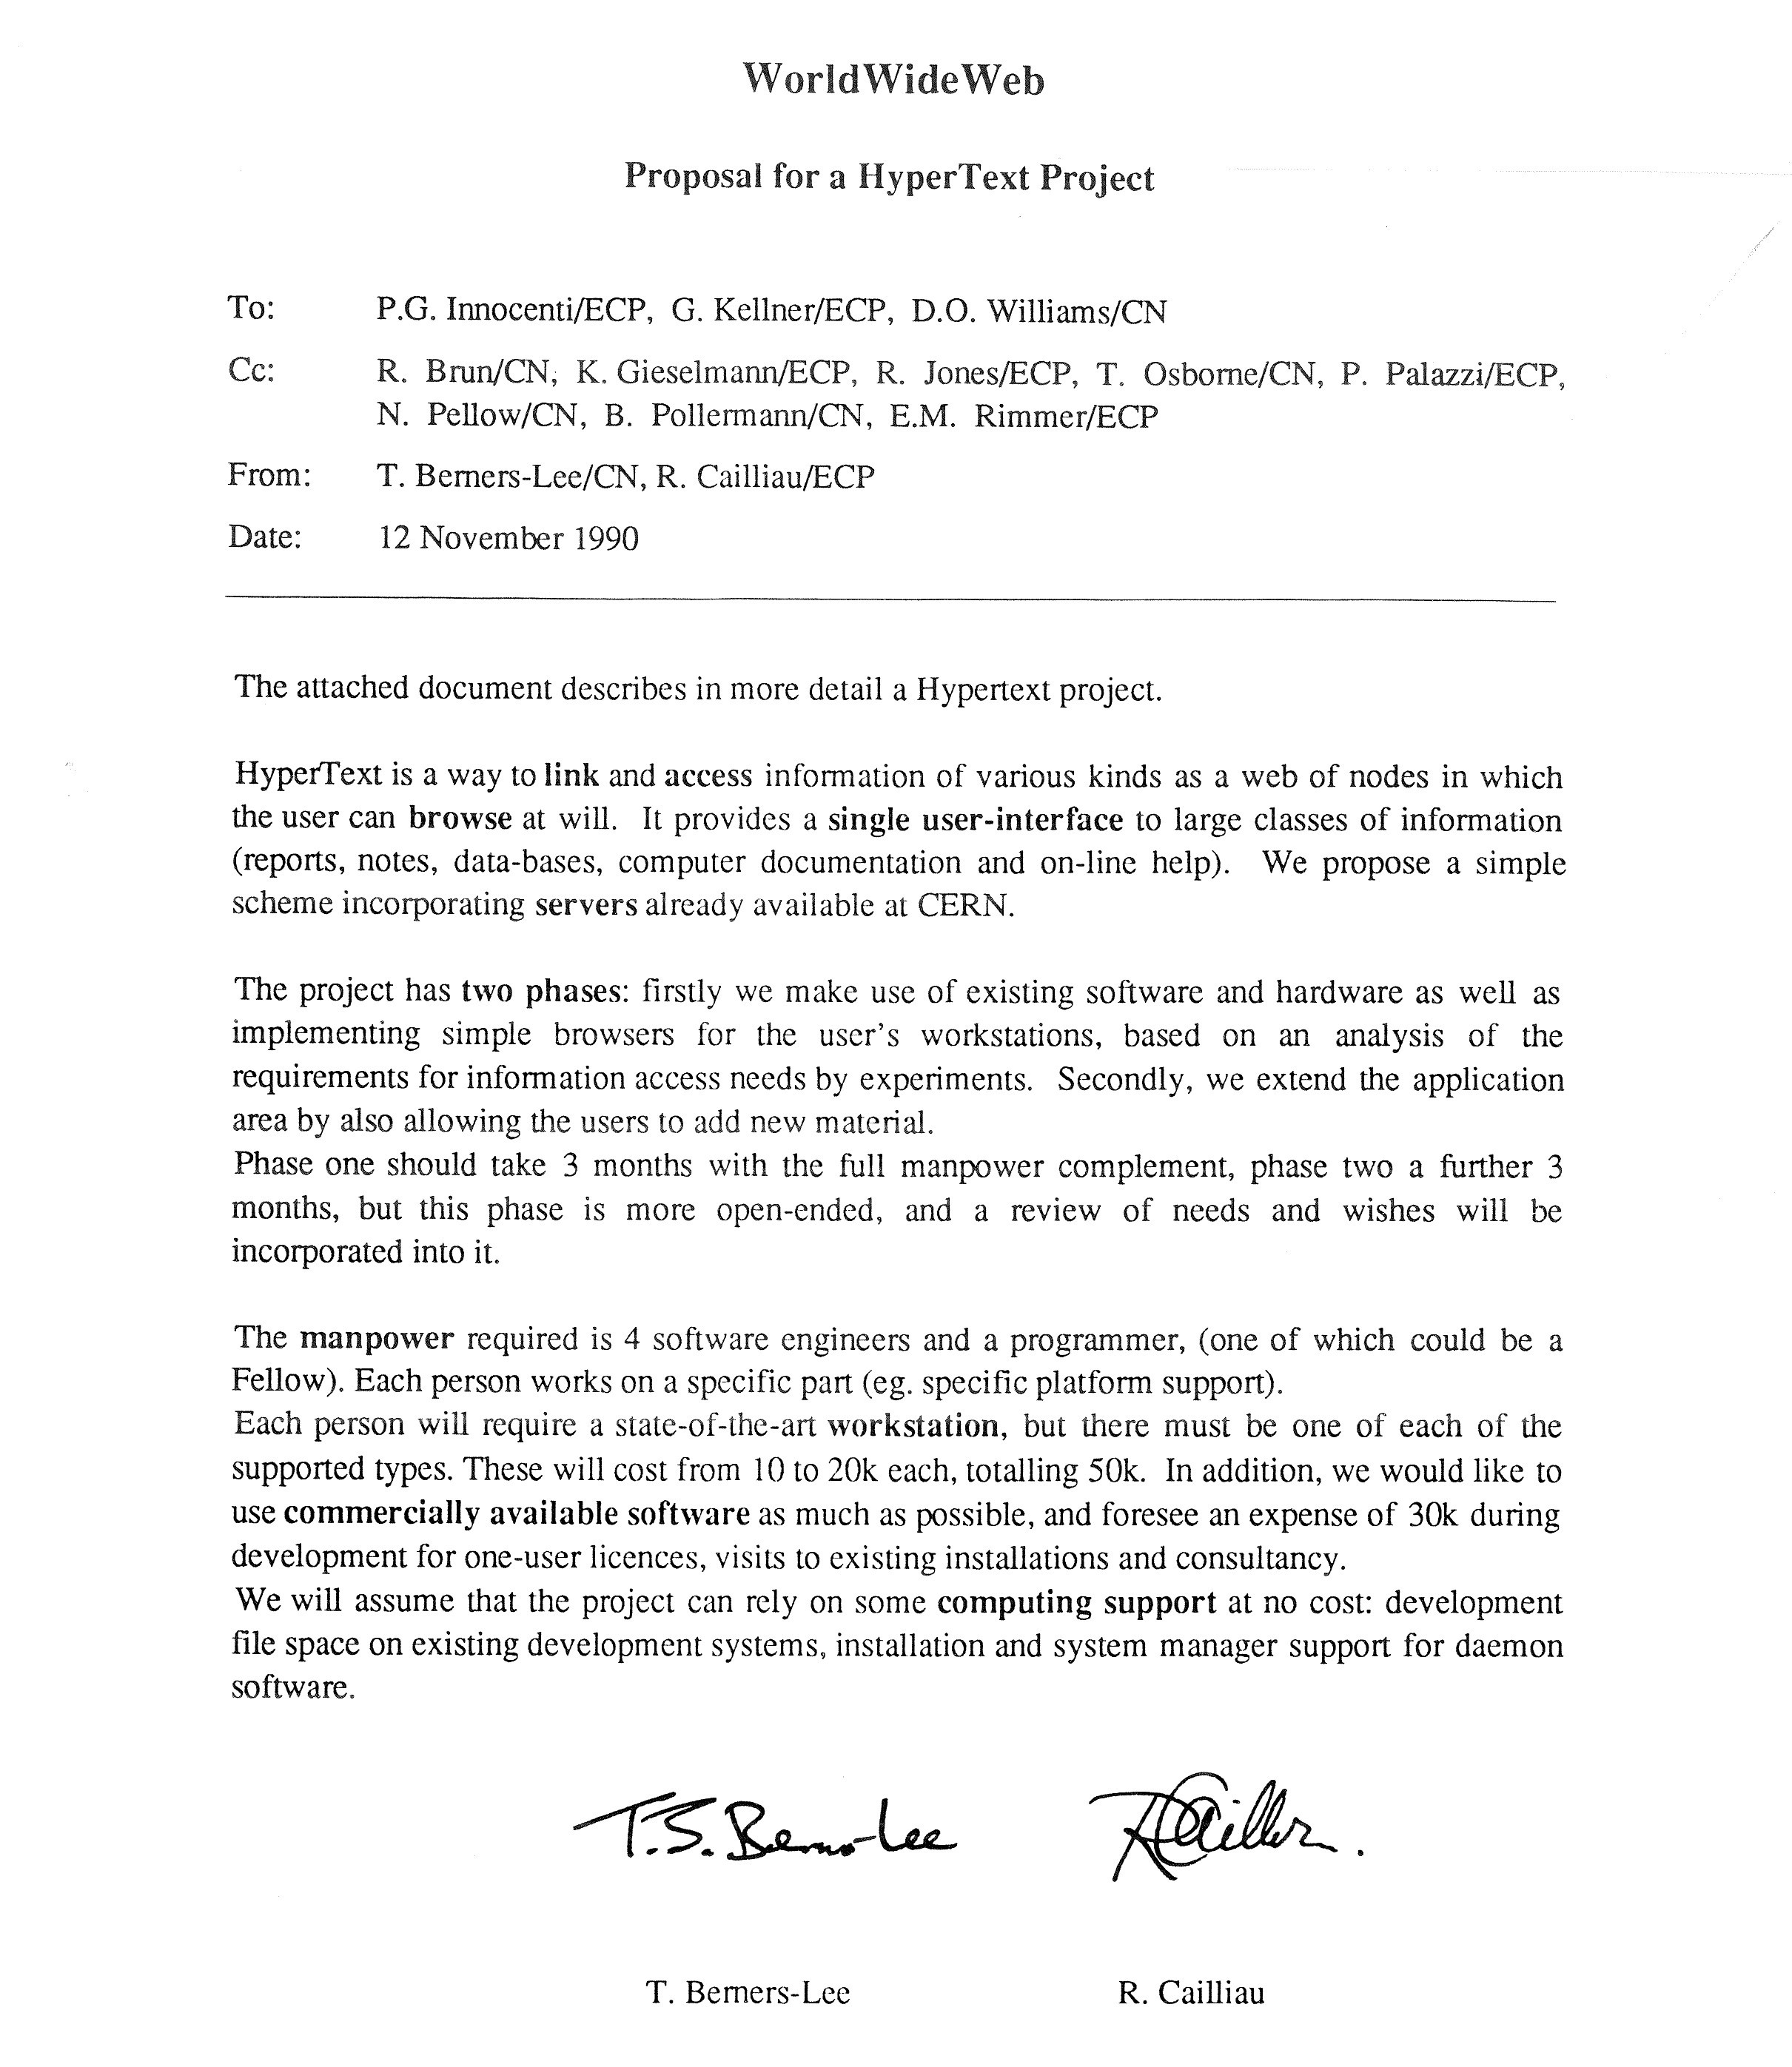
\includegraphics[width=1.0\textwidth]{images/proposta-web-1990.jpg}
    \caption{Prima pagina del documento di formalizzazione per il World Wide Web}
    \label{fig:proposta1990}
    \cite{formalizzazione1990}
\end{figure}
\FloatBarrier % per far si che ciò che scrivo successivamente appaia dopo le immagini


\section{L'evoluzione del web e la sua diffusione}
Inizialmente solo pochi utenti avevano accesso alla piattaforma informatica su cui girava il primo browser, nel quale era possibile fare ricerche solo per parole chiave dato che i motori di ricerca non esistevano ancora. Perciò si decise di sviluppare un browser più semplice che funzionava solo in modalità di linea, affinché funzionasse su ogni sistema.
Alla fine del 1991 negli Stati Uniti venne messo in rete il primo server web in un laboratorio di fisica.\\
A questo punto esistevano due tipi di browser:
\begin{itemize}
    \item La versione originale (Figura \ref{fig:browserOriginale}), la quale funzionava solo sulle macchine NeXT. \footnote{Uno dei primi computer di Steve Jobs, sul quale veniva eseguito il primo browser web.}
    \item La versione in modalità di linea (Figura \ref{fig:browserCommandLine}), la quale era più facile da installare ed eseguire su qualsiasi piattaforma, ma limitata in termini di potenza e facilità d'uso.
\end{itemize}
Date le grandi dimensioni del progetto, il team del CERN non poteva fare tutto il lavoro da solo. Perciò Berners-Lee lanciò un appello via internet al fine di trovare nuovi sviluppatori che si unissero allo sviluppo di questa rivoluzionaria tecnologia.

All'inizio del 1993 iniziarono a nascere diversi browser, che funzionavano sia in ambienti PC e Macintosh. La nascita di browser affidabili e facili da usare, comportarono una diffusione immediata del World Wide Web.

Il 1994 fu considerato \textit{"l'anno del web"} e al suo termine il Web contava 10.000 server, di cui 2.000 commerciali, e 10 milioni di utenti.\cite{historyOfWeb}
\\

\begin{figure}[h]
\begin{subfigure}{0.5\textwidth}
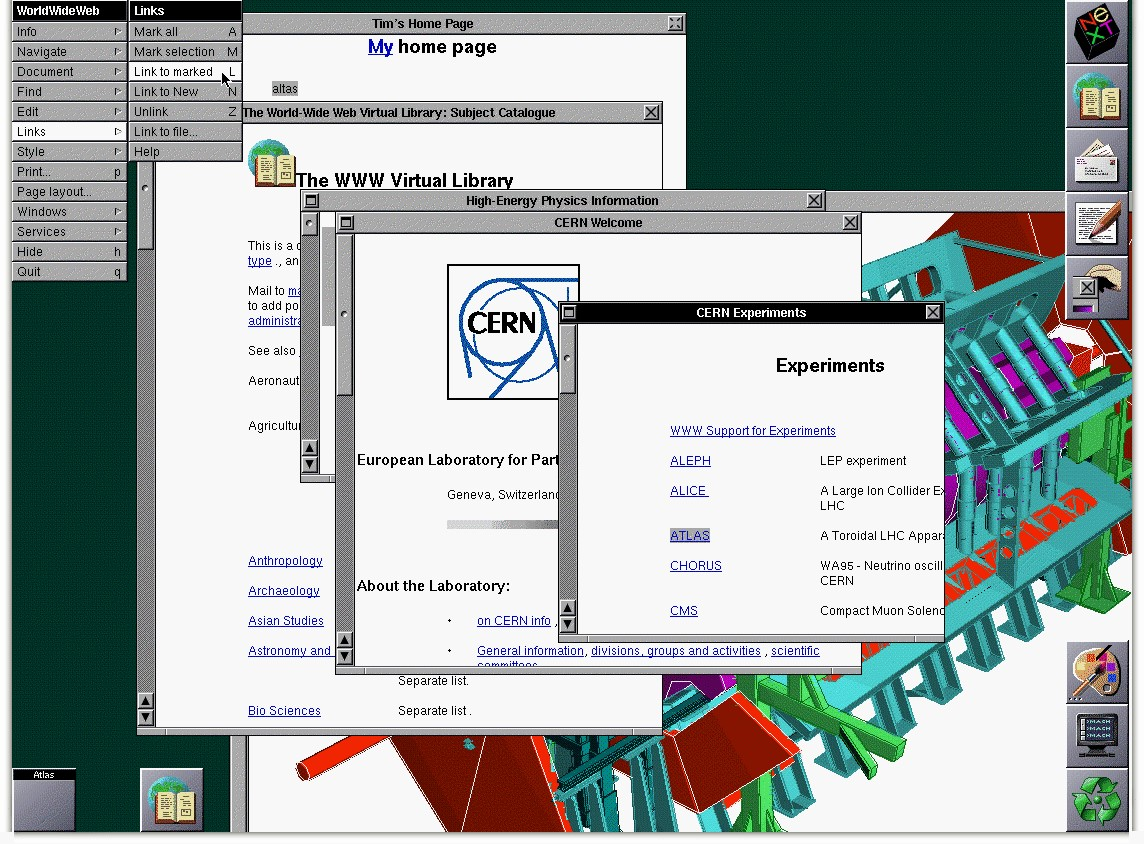
\includegraphics[width=\textwidth]{images/primo browser.jpg} 
\caption{Browser originale con interfaccia grafica}
\label{fig:browserOriginale}
\cite{primoBrowser}
\end{subfigure} \hspace*{\fill}
\begin{subfigure}{0.5\textwidth}
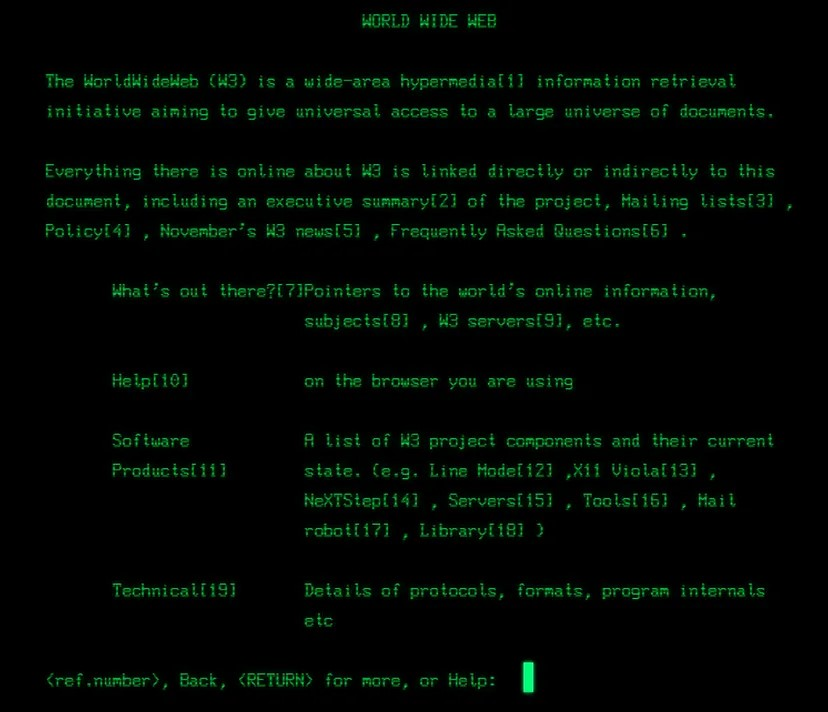
\includegraphics[width=\textwidth]{images/primo browser command line.jpg}
\caption{Browser a linea di comando}
\label{fig:browserCommandLine}
\cite{browserLineaDiComando}
\end{subfigure}

\caption{I primi due tipi di browser sviluppati nel 1991}
\label{fig:image2}
\end{figure}
\newpage
\subsection{Una tecnologia alla portata di tutti}
Gli sviluppatori al CERN decisero fin da subito che il web dovesse essere utilizzabile da tutti e che nessuno dovesse rinchiuderlo in un sistema proprietario. Per questo motivo il CERN decise di presentare una proposta, che fu subito accettata, alla commissione dell'Unione Europea al fine di formare un consorzio internazionale in collaborazione con il Massachussets Institute of Technology (MIT).

Nel 1994 Tim Berners-Lee lasciò il CERN per unirsi al MIT e fondò l'International World Wide Consortium (W3S), il quale al giorno d'oggi definisce i vari standard nello sviluppo web e di applicazioni.

Ad oggi gli standard web del W3S garantiscono un'ottimizzazione per l'interoperabilità\footnote{L'interoperabilità è, in ambito informatico, la capacità di un sistema o di un prodotto informatico di cooperare e di scambiare informazioni o servizi con altri sistemi o prodotti in maniera più o meno completa e priva di errori, con affidabilità e con ottimizzazione delle risorse.\cite{interoperabilità} \\}, la sicurezza e privacy dei dati, accessibilità e l'internazionalizzazione\footnote{L'internazionalizzazione in economia, e per estensione in informatica e altri ambiti, è il processo di adattamento di una impresa, un prodotto, un marchio, pensato e progettato per un mercato o un ambiente definito, ad altri mercati o ambienti internazionali, in modo particolare altre nazioni e culture.\cite{internazionalizzazione}}.
\\

\textit{"Web standards are blueprints or building blocks of a consistent and harmonious digitally connected world. They are implemented in browsers, blogs, search engines, and other software that power our experience on the web."}\cite{w3sStandard}

\textit{\hspace{14.2cm}- W3S}
\newpage
\section{Architettura client-server}
Un sistema client-server utilizza un'architettura nella quale un client, che è responsabile dell'interazione con l'utente e solitamente è un'interfaccia grafica di limitata complessità, si connette ad un server, il quale implementa la logica del sistema e tutte le tecniche per la gestione degli accessi, allocazione, rilascio e sicurezza delle risorse, per la fruizione di un determinato servizio, come ad esempio la condivisione di una certa risorsa.\cite{clientServer1}\cite{clientServer2}

I vantaggi di un'architettura di questo tipo sono:\cite{clientServerVantaggi}
\begin{itemize}
    \item Accessibilità dei dati: dato che il server mantiene i dati in una posizione centralizzata, più utenti possono accedere e lavorare simultaneamente sui dati garantendone una maggiore condivisione.
    \item Scalabilità: è possibile aggiornare il server ad una macchina più potente, senza cambiamenti visibili all'utente. Ciò garantisce anche la possibilità di introdurre nuove tecnologie, sia hardware che software.
    \item Integrità dei dati: il server può usufruire e fornire di servizi che garantiscono la protezione dei dati, archiviazione crittografata di file.
\end{itemize}
%\newpage
\subsection{Protocollo HTTP}
Il protocollo HTTP, il quale utilizza uno schema client-server, è una delle tecnologie alla base del web.
Quando usiamo un browser per caricare una pagina web, esso agisce come client HTTP comunicando con un server HTTP.\cite{protocolloHTTP}
\begin{figure}[h]
    \centering
    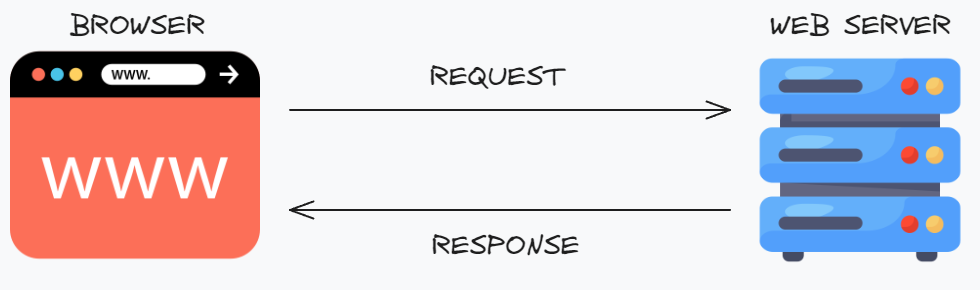
\includegraphics[width=1.0\textwidth]{images/request response.png}
    \caption{Comunicazione tra web-browser e web-server}
    \label{fig:request-response}
\end{figure}

Ad esempio, come vedremo più nello specifico nel capitolo \ref{capitolo-4}, nel momento in cui un utente vuole caricare la pagina per visualizzare i postit (Figura \ref{fig:request-response}):  
\begin{enumerate}
    \item Il browser aprirà una connessione verso il server, inviando una richiesta (request).
    \item Ricevuta la richiesta, il server si occuperà di gestire la logica di recupero dei dati richiesti, inviandoli in risposta (response) a chi ha fatto la richiesta.
    \item Il browser gestirà la risposta reindirizzando e caricando il contenuto nella pagina del sito.
\end{enumerate}